\documentclass[a4paper, 11pt]{article}

\usepackage[a4paper,margin=1in]{geometry}
\usepackage[english]{babel}
\usepackage[utf8]{inputenc}
\usepackage[T1]{fontenc}
\usepackage[superscript,biblabel]{cite}
\usepackage[toc,page]{appendix}
\usepackage{lmodern}
\usepackage{listings}
\usepackage{graphicx}
\usepackage{amsmath}
\usepackage{framed}
\usepackage{amsfonts}
\usepackage{caption}
\usepackage{subcaption}
\usepackage{listings}
\usepackage{tabularx}
\usepackage{color}
\usepackage[dvipsnames]{xcolor}
\usepackage{fancyhdr}
\usepackage{lastpage}
\usepackage{hyperref}
% \usepackage{tcolorbox}
\usepackage{dirtytalk}
\usepackage{tikz}

\widowpenalties 1 10000

\usetikzlibrary{matrix}


\graphicspath{{imgs/}}


\definecolor{morange}{RGB}{237,106,90}
\definecolor{mgreen}{RGB}{63,127,95}
\definecolor{mpurple}{RGB}{127,0,85}

\lstset{
  basicstyle=\small\ttfamily, % Global Code Style
  captionpos=b, % Position of the Caption (t for top, b for bottom)
  extendedchars=true, % Allows 256 instead of 128 ASCII characters
  tabsize=2, % number of spaces indented when discovering a tab
  columns=fixed, % make all characters equal width
  keepspaces=true, % does not ignore spaces to fit width, convert tabs to spaces
  showstringspaces=false, % lets spaces in strings appear as real spaces
  breaklines=true, % wrap lines if they don't fit
  frame=trbl, % draw a frame at the top, right, left and bottom of the listing
  frameround=tttt, % make the frame round at all four corners
  framesep=4pt, % quarter circle size of the round corners
  numbers=left, % show line numbers at the left
  numberstyle=\tiny\ttfamily, % style of the line numbers
  commentstyle=\color{mgreen}, % style of comments
  keywordstyle=\color{mpurple}, % style of keywords
  stringstyle=\color{morange}, % style of strings
}

% TAILLE DES PAGES (A4 serré)

\setlength{\parindent}{0pt}
\setlength{\parskip}{1em}
%% \setlength{\textwidth}{17cm}
%% \setlength{\textheight}{24cm}
%% \setlength{\oddsidemargin}{-.7cm}
%% \setlength{\evensidemargin}{-.7cm}
%% \setlength{\topmargin}{-.5in}


\pagestyle{fancy}
\renewcommand{\headrulewidth}{0pt}
\renewcommand{\footrulewidth}{0.6pt}% default is 0pt
\lhead{}
\rhead{}
\lfoot{Page \thepage}
% \lfoot{Page \thepage\ of \pageref{LastPage}}
\rfoot{Rémi Lespinet, Victor Busa}
\cfoot{}
\cfoot{}



\newcounter{cquestion}
\renewcommand{\thecquestion}{\arabic{cquestion}}
\newenvironment{question}
{\par \vspace{0.5em} \noindent \stepcounter{cquestion} \hspace{-1em}
 $\bullet$ \underline{Q\thecquestion :}}
{}

\newenvironment{note}
{\begin{framed} \textbf{Note : }}
{\end{framed}}


% Commandes de mise en page
\newcommand{\file}[1]{\lstinline{#1}}
\newcommand{\name}[1]{\emph{#1}}
\newcommand{\Fig}[1]{Fig \ref{#1} p. \pageref{#1}}
\newcommand{\Figure}[1]{Figure \ref{#1} p. \pageref{#1}}
\newcommand{\Tab}[1]{Tab \ref{#1} p. \pageref{#1}}
\newcommand{\Table}[1]{Table \ref{#1} p. \pageref{#1}}
\newcommand{\itemi}{\item[$\bullet$]}
% Commandes color
\newcommand{\colgood}[1]{\color{ForestGreen} #1}
\newcommand{\colbad}[1]{\color{BrickRed} #1}


% Commandes de maths
\newcommand{\function}[3]{#1 : #2 \to #3}
\newcommand{\intn}[2]{\left\{ #1 \dots #2 \right\}}
\newcommand{\intr}[2]{\left[ #1 ; #2 \right]}
\newcommand{\intro}[2]{\left] #1 ; #2 \right[}
\newcommand{\dotp}[2]{\langle #1, #2 \rangle}
\newcommand{\logn}[1]{\ln\left( #1\right)}
%% \newcommand{\det}[1]{\left| #1 \right|}
\newcommand{\pd}[2]{\frac{\partial #1}{\partial #2}}
\newcommand{\norm}[1]{\|#1\|}
\newcommand{\set}[2]{\left\{ #1 \hspace{.5em} ; \hspace{.5em}#2 \right\}}
\newcommand{\tr}[1]{Tr\left( #1 \right)}
\newcommand{\pcond}[2]{p(#1 \hspace{-.2em}\mid\hspace{-.2em} #2)}


\newcommand{\iid}{i.i.d }
\newcommand{\wrt}{w.r.t }

% Commandes informatique
\newcommand{\pfun}[1]{{\textbf{\texttt{#1}}}}

\newcommand{\ipart}[1]{\vspace{0.5em}\textbf{#1}\vspace{0.5em}}



\pagenumbering{arabic}

\title{\textsc{Unsupervised Learning - MVA 2017/2018 \\ \emph{Homework 1}} }
\author{Victor Busa, Rémi Lespinet}
\date{}

\begin{document}

\maketitle
\thispagestyle{fancy}

\section{Low rank Matrix Completion}

The low rank matrix completion (LRMC) has been implemented in python3
using the numpy library.

% \subsection{Choice of the stopping criterion}

% As presented in the lesson, the algorithm must stop when
% \begin{equation*}
%   \mathcal{P}_\Omega(X - A) \approx 0
% \end{equation*}
% Hence, we can take any norm and use
% \begin{equation*}
%   \norm{\mathcal{P}_\Omega(X - A)} < \epsilon
% \end{equation*}
% as a stopping criterion. We tried the infinite norm, the frobenius
% norm


\section{Face completion}

% There's a lot of ways we can build a matrix from several images, some
% of them making more sense than other. For this exercice, we have tried
% several of them, which are presented in the following sections.

% \subsection{Image seen as a point in $\mathbb{R}^{W \times H}$}

We know that the intensity of light reflected on a lambertian surface
under a varying light source position (with one source) leaves in a
space of dimension 3 :
\begin{equation*}
  I_D(x,y,z) = L(x, y, z) \cdot N(x,y,z) C I_L
\end{equation*}
where $L(x, y, z)$ is the light direction vector pointing from the
point on the surface to the light source, $N$ is the normal of the
surface in that point, $C$ is the color of the light source and $I_L$
is the intensity of the light source.


In our case, we have faces under a varying illumination source. These
are of course not lambertian surfaces (even if we forget about self
shadowing, skin is a very complicated material to model). Still it
provides the intuitition that the matrix obtained by stacking the
images seen as vectors (vectors of size $192 \times 168 = 32256$, thus
forming a matrix of size $32256 \times 10$) is low rank.

For each pixel we remove the pixel with probability $\rho$ (Bernoulli
random variable), and we use this matrix as input in the LRMC
algorithm. The figure \ref{fig:yale-full-size} present the results
(showing only the first image of the dataset), for different values of
$\tau$ and different values of $\rho$. (The full reconstruction for the
$10$ images figures for the same values of $\tau$ are shown on the
appendix, figures \ref{fig:mse20}, \ref{fig:mse40}, \ref{fig:mse60},
\ref{fig:mse80})


\begin{figure}[p]
  \centering
  \begin{subfigure}[t]{0.90\textwidth}
    \centering
    \includegraphics[width=\textwidth]{yale_192_168_oneface_original}
    \vspace{-2.0em}\caption{Faces images with (10\%, 20\%, 40\% 60\% and 80\%) of
      missing entries}\label{fig:yale-192-168-oneface-original}
  \end{subfigure}
  \vskip\baselineskip\vspace{-1.0em}
  \begin{subfigure}[t]{0.90\textwidth}
    \centering
    \includegraphics[width=\textwidth]{yale_192_168_oneface_1000}
    \vspace{-2.0em}\caption{Faces images reconstructed by convex optimization with
      $\tau = 10^3$}\label{fig:yale-192-168-oneface-1000}
  \end{subfigure}
  \vskip\baselineskip\vspace{-1.0em}
  \begin{subfigure}[t]{0.90\textwidth}
    \centering
    \includegraphics[width=\textwidth]{yale_192_168_oneface_20000}
    \vspace{-2.0em}\caption{Faces images reconstructed by convex optimization with
      $\tau = 2 \cdot 10^4$}\label{fig:yale-192-168-oneface-20000}
  \end{subfigure}
  \vskip\baselineskip\vspace{-1.0em}
  \begin{subfigure}[t]{0.90\textwidth}
    \centering
    \includegraphics[width=\textwidth]{yale_192_168_oneface_400000}
    \vspace*{-2.0em}\caption{Faces images reconstructed by convex optimization with
      $\tau = 4 \cdot 10^5$}\label{fig:yale-192-168-oneface-400000}
  \end{subfigure}
  \vskip\baselineskip\vspace*{-1em}
  \begin{subfigure}[t]{0.90\textwidth}
    \centering
    \includegraphics[width=\textwidth]{yale_192_168_oneface_8000000}
    \vspace{-2.0em}\caption{Faces images reconstructed by convex optimization with
      $\tau = 8 \cdot 10^6$}\label{fig:yale-192-168-oneface-8000000}
  \end{subfigure}
  \caption{Reconstruction of the first face of the Yale dataset using
    the LRMC algorithm on 10 images of the set ($192 \times 168$) for
    different values of $\rho$ and $\tau$}\label{fig:yale-full-size}
\end{figure}


As $\tau$ increases, we see that we are able to recover better the
image (the MSE decreases and we can see it visually). This is not
suprising since the relaxed problem we want to solve look like

\begin{equation*}
\begin{aligned}
& \underset{A}{\text{minimize}}
& & \norm{A}_* \\
& \text{subject to}
& & P_\Omega(A)= P_\Omega(X)
\end{aligned}
\end{equation*}

And the problem we are actually solving with LRMC is
\begin{equation}
\begin{aligned}
& \underset{A}{\text{minimize}}
& & \tau \norm{A}_* + \dfrac{1}{2}\norm{A}^2_F \\
& \text{subject to}
& & P_\Omega(A)= P_\Omega(X)
\end{aligned}
\tag{$\star$}
\label{eq:min-reg-relaxed}
\end{equation}

Hence, the larger $\tau$, the more the solution of LRMC approximates
well our original problem.  If $\tau$ is small, the problem becomes
equivalent to

\begin{equation*}
\begin{aligned}
& \underset{A}{\text{minimize}}
& & \norm{A}^2_F \\
& \text{subject to}
& & P_\Omega(A)= P_\Omega(X)
\end{aligned}
\end{equation*}

Which admits the trivial solution
\begin{equation*}
  A(i, j) = \left\{
    \begin{array}{ll}
      X(i, j) & \text{ if } (i, j) \in \Omega \\
      0 & \text{ otherwise}
    \end{array}
    \right.
\end{equation*}


\begin{figure}[h]
  \centering
  \includegraphics[width=.8\linewidth]{curves_pt}
  \caption{Mean-squared-error for different value of $\tau$ function
    of the percentage of missing entries (for the 10 images
    $(192 \times 168)$ suggested of the first person in the yale
    dataset)}
  \label{fig:curves}
\end{figure}


% \begin{figure}[h]
%   \centering
%   \includegraphics[width=.6\linewidth]{table}
%   \caption{Reported mean-squared-error for different value of $\tau$ function
%     of the percentage of missing entries (for the 10 images
%     $(192 \times 168)$ suggested of the first person in the yale
%     dataset)}
%   \label{fig:table}
% \end{figure}



The figure \ref{fig:curves} represent the observed MSE as a function
of the number of missing entries $\rho$ for different values of
$\tau$.  % Figure \ref{fig:table} shows the correspondings numerical
% values.


The results are good, but looking at the book
\hspace{0.3em}\cite{vidal} (figure \ref{fig:faces-book}), we see that
it has better results for the same values of $\tau$ and $\rho$. To
obtain similar results, we took the whole \name{yaleB20} of the
\emph{Extended Yale Face Database B}\hspace{.3em} \cite{yale} ($64$
images), resized all the images by $50\%$, and ran the exact same
procedure with these $64$ images of size $96 \times 84$. The results
obtained are represented in figure \ref{fig:yale-reduced-size}

\begin{figure}[h]
  \centering
  \includegraphics[width=0.7\linewidth]{img_book}
  \caption{First row: Face images with (30, 50, 70, 80, 90)\% of
    missing entries, second to last rows: Face images reconstructed
    for $\tau$ being respectively (1e3, 2e4, 4e5, 8e6)}
  \label{fig:faces-book}
\end{figure}


\begin{figure}[p]
  \centering
  \begin{subfigure}[t]{0.90\textwidth}
    \centering
    \includegraphics[width=\textwidth]{yale_96_84_oneface_original}
    \vspace{-2.0em}\caption{Faces images with (30\%, 50\%, 70\% 80\% and 90\%) of
      missing entries}\label{fig:yale-192-168-oneface-original}
  \end{subfigure}
  \vskip\baselineskip\vspace{-1.0em}
  \begin{subfigure}[t]{0.90\textwidth}
    \centering
    \includegraphics[width=\textwidth]{yale_96_84_oneface_1000}
    \vspace{-2.0em}\caption{Faces images reconstructed by convex optimization with
      $\tau = 10^3$}\label{fig:yale-192-168-oneface-1000}
  \end{subfigure}
  \vskip\baselineskip\vspace{-1.0em}
  \begin{subfigure}[t]{0.90\textwidth}
    \centering
    \includegraphics[width=\textwidth]{yale_96_84_oneface_20000}
    \vspace{-2.0em}\caption{Faces images reconstructed by convex optimization with
      $\tau = 2 \cdot 10^4$}\label{fig:yale-192-168-oneface-20000}
  \end{subfigure}
  \vskip\baselineskip\vspace{-1.0em}
  \begin{subfigure}[t]{0.90\textwidth}
    \centering
    \includegraphics[width=\textwidth]{yale_96_84_oneface_400000}
    \vspace*{-2.0em}\caption{Faces images reconstructed by convex optimization with
      $\tau = 4 \cdot 10^5$}\label{fig:yale-192-168-oneface-400000}
  \end{subfigure}
  \vskip\baselineskip\vspace*{-1em}
  \begin{subfigure}[t]{0.90\textwidth}
    \centering
    \includegraphics[width=\textwidth]{yale_96_84_oneface_8000000}
    \vspace{-2.0em}\caption{Faces images reconstructed by convex optimization with
      $\tau = 8 \cdot 10^6$}\label{fig:yale-192-168-oneface-8000000}
  \end{subfigure}
  \caption{Reconstruction of the same face of the book
    \ref{fig:faces-book} (on the Yale dataset) using the LRMC
    algorithm on 64 images ($96 \times 84$) of this face under
    different illuminations for different values of $\rho$ and
    $\tau$}\label{fig:yale-reduced-size}
\end{figure}


% \begin{figure}[h]
%   \centering
%   \includegraphics[width=1.0\textwidth]{yale_reduced_size_4t_5p}
%   \caption{Ouptut of the LRMC algorithm for different value of $\tau$
%     and $\rho$ on the reduced images ($96 \times 84$) of the yale
%     dataset}\label{fig:yale-reduced-size}
% \end{figure}

The results are better both visually and in term of MSE. This shows
that the higher the number of image, the better the algorithm
reconstructs (if we forget for the fact that we resized the image for
speed reasons). This is intuitive, and theoritically, Here, the
expected number of observed entries $M$ is
\begin{equation*}
  M = (1 - \rho) N D
\end{equation*}

Hence the theorem presented in the class can be expressed in the
following form : there exist a constant c such that if
\begin{equation*}
  (1 - \rho) \ge c \nu^4 \dfrac{d}{D} \left( \log(N) \right)^2
\end{equation*}
then the images are recovered with porbability at least $1 - N^{-3}$

Which means that if we increase $D$ (we add new images), we can take a
higher $\rho$ and still verify the equality

\ipart{Choice of $\beta$}

As suggested in the subject, we chose $\beta$ as
\begin{equation*}
  \beta = \min{\left( 2, \dfrac{N D}{M} \right)} = \min{\left( 2, \dfrac{1}{1 - \rho} \right)}
\end{equation*}
This makes sense because the algorithm provably converges
\hspace{.3em}\cite{svt} to the solution of the minimization problem
\eqref{eq:min-reg-relaxed} if
\begin{equation*}
  0 < \beta < 2
\end{equation*}

% \subsection{Image seen as W points in $\mathbb{R}^H$}

% We have also tried to compute the matrix differently, even if we don't
% know if the matrix is really low rank.

% TODO

\clearpage
\section{Movie Recommendation Grand Challenge}

For the Movie recommendation challenge, we want to apply the same
algorithm. We build the matrix $X$ such that $X(i, j)$ corresponds to
the rating that the user $i$ has given to the movie $j$.

Intuitively, the fact that the matrix is low rank can be explained by
the fact that every user is a combination of a small number of
\say{eigen-users}, that is there's a small there's a small number of
\say{behaviors}. This assumption is not totally absurd, and it makes
sense to try to recover the full matrix of ranking using this method.

This situation is different than the previous one, in which we
artifially removed entries in the image, and hence we did know the
real values of the missing entries. In this case we do not have access
to the real matrice (in that sense, this is a more realistic
situation). To compute the MSE, we remove 10\% of the known entries,
give that as input to LRMC, and look at these 10\% entries to compute
the MSE. To have more accurate results, we use cross-validation : we
randomly create a partition of size 10 of the missing entries and
calculate the mean MSE over the elements of the partition.

The results are reported in the table \ref{tab:mse-movies}


\begin{table}[h!]
  \centering
  \begin{tabular}{| c | c | c | c | c |}
    \hline
    $\tau$ & 100 & 500 & 2500 & 12500 \\
    \hline
    Horror  & 5.33 & 2.72 & 1.81 & 1.59 \\
    Romance & 5.28 & 2.94 & 2.09 & 1.91 \\
    Both    & 5.51 & 2.83 & 1.88 & 1.63 \\
    \hline
  \end{tabular}
  \captionof{table}{Mean square error obtained for the horror and
    romance categories for different values of $\tau$ (obtained with
    cross-validation by the procedure described
    above)} \label{tab:mse-movies}
\end{table}

As seen in the previous case, increasing the value of $\tau$ leads to
a lower MSE, but also requires a higher number of iterations. In our
experiment, the number of iterations is capped to $1000$. For our
choice of the norm, we always reach the maximum number of iteration,
and never terminate due to the stopping criterion. This might explain
the results

For this reason, we have tried to improve the algorithm (see
\ref{sec:ameliorations}).


The figure \ref{fig:movies_challenge_mse} shows the evolution of the
MSE with $\tau$ (computed with cross-validation by the method
described above).
\begin{figure}[h]
  \centering
  \includegraphics[width=.8\textwidth]{movies_challenge_mse}
  \caption{Ouptut of the LRMC algorithm for different value of $\tau$ and
    $\rho$}\label{fig:movies_challenge_mse}
\end{figure}


\section{Ameliorations}
\label{sec:ameliorations}



\subsection{Algorithm speed}

In this algorithm, the time performance entirely relies only on the
SVD computation. Fortunately, high number of missing entries
corresponds to sparse matrices and hence the SVD can be computed more
easily.  We did the implementation in python, and we could not use
this potentential at maximum. Moreover, with the tested stopping
criterion, the algorithm was always stopped by the maximum number of
iterations, and taking a very high number of iterations lead to some
numerical problems.  We were very interested in knowing if we could
improve the result, so we decided first to use Scikit-CUDA or even
TensorFlow to do calculations, but it appeared that not only there is
no efficient parallel implementation of the SVD on GPU, but also that
the CPU implementation is higly optimized (aka MKL Intel), and hence
hard to outperform. We also did a $C++$ implementation of the
algorithm, hoping that the SVD would be much faster in this
language. We use the \name{Eigen3} library (not included in the
archive) for linear algebra calculations, and the \name{REDSVD}
library to compute the SVD.  nfortunately, it appears that our
implementation is not really faster, and we did not have the time to
improve it before the deadline... We have included this code in the
archive anyway.

In this algorithm, we only care about the singular values that are
above $\tau$ in the singular value decomposition, and since it appears
that some SVD algorithms can compute very efficiently the $d$ largest
singular values. A proposed method \cite{svt} to increase efficiency
would be to compute the $d$ largest singular values, and then
iteratively increase $d$ up to the point where the lowest singular
value returned is less than $\tau$. At this point, it is not necessary
to compute the other singular values, since they will all be zero
after the thresholding, hence it is only necessary to compute a
smaller part of the $U$ and $V$ matrices of the singular value
decomposition.

We might also get better results by starting the algorithm with the
value of $A$ computed for a lower value of $\tau$.

\subsection{Using a decay learning rate}

Decreasing the learning rate over time can both lead to better or
worse performance. Actually it is very hard to determine how to
decrease the learning rate over time.%  as the decreasing rate both
% depends on the matrix of missing entries $W$ and \textbf{on the
%   percentage of missing entries}. (See tables
% \ref{tab:decay_learning_rate} and
% \ref{tab:decay_learning_rate2}).

Here we choose to decrease the learning rate if the mean-squared-error
computed after updating A is higher than the mean-squared-error before
updating A. In python it corresponds to:

% \begin{tcolorbox}
\begin{lstlisting}
fro_prev = mse(X, A, W)
...
fro = mse(X, A, W)
if (fro > fro_prev):
	beta *= 0.9
\end{lstlisting}
% \end{tcolorbox}

\begin{table}[h]
\centering
\begin{tabular}{|c|c|c|c|c|}
\hline
learning rate & run 1 & run 2 & run3 & run4 \\ \hline
no decay & 45.6 & 49.6 & 40.5 & 39.6 \\ \hline
decay by 0.9 & 54.6 & 71.1 & 49 & 51.7 \\ \hline
\end{tabular}
\caption{For $\tau$ = 4e5 and 40 \% of missing entries}
\label{tab:decay_learning_rate}
\end{table}

\begin{table}[h]
\centering
\begin{tabular}{|c|c|c|c|c|}
\hline
learning rate & run 1 & run 2 & run3 & run4 \\ \hline
no decay & 283 & 296 & 330 & 282 \\ \hline
decay by 0.9 & 235 & 252 & 245 & 268 \\ \hline
\end{tabular}
\caption{For $\tau$ = 2e4 and 80 \% of missing entries}
\label{tab:decay_learning_rate2}
\end{table}

As we can see on the tables above, sometimes using a decay learning
can lead to better final mean-squared-errors (Table
~\ref{tab:decay_learning_rate2}), while it can also leads to worst
performance as shown in Table ~\ref{tab:decay_learning_rate}. On
average it appears that tuning the rate by which we want to decay the
parameter $\beta$ is a really difficult task as $\beta$ both depends
on the number of missing entries and on the disposition of these
entries in $W$. Here, decreasing the learning rate doesn't lead to
better performance \textbf{on average}. The only interest is that it
allows the algorithm to stop earlier in its process and thus take less
time to terminate. This method is not applicable to the third exercise
as the matrix $X$ is already sparse.

\section{Conclusion}

We both implemented the algorithm entirely, this allowed us to verify
our results (the two codes are availables in the \file{src}
directory).  When everything was working properly, Victor Busa tried
to use TensorFlow for computing the SVD more efficiently, experimented
decay on the learning rate. Rémi Lespinet adapted the code in
\name{C++}. Since we obtain the same results for both implementations,
figures come from either one or the other. For the redaction of this
report, we both wrote a draft version on our side, that we later
merged to produce this document.

% We both did the homework entirely, and we merged everything after that,
% hence


\clearpage

\begin{figure}[p]
  \centering
  \includegraphics[width=0.9\linewidth]{mse_20}
  \caption{images reconstruction for \textbf{20\% of missing
      entries}. The first row corresponds to the corrupted images, the
    second to last rows correspond to the reconstruction for $\tau$
    being \{1e3, 2e4, 4e5, 8e6\} respectively}
  \label{fig:mse20}
\end{figure}
\begin{figure}[p]
  \centering
  \includegraphics[width=0.9\linewidth]{mse_40}
  \caption{\small{images reconstruction for \textbf{40\% of missing
      entries}. The first row corresponds to the corrupted images, the
    second to last rows correspond to the reconstruction for $\tau$
    being \{1e3, 2e4, 4e5, 8e6\} respectively}}
  \label{fig:mse40}
\end{figure}

\begin{figure}[p]
  \centering
  \includegraphics[width=0.9\linewidth]{mse_60}
  \caption{images reconstruction for \textbf{60\% of missing
      entries}. The first row corresponds to the corrupted images, the
    second to last rows correspond to the reconstruction for $\tau$
    being \{1e3, 2e4, 4e5, 8e6\} respectively}
  \label{fig:mse60}
\end{figure}

\begin{figure}[p]
  \centering
  \includegraphics[width=0.9\linewidth]{mse_80}
  \caption{images reconstruction for \textbf{80\% of missing
      entries}. The first row corresponds to the corrupted images, the
    second to last rows correspond to the reconstruction for $\tau$
    being \{1e3, 2e4, 4e5, 8e6\} respectively}
  \label{fig:mse80}
\end{figure}

\clearpage
\begin{thebibliography}{9}
\bibitem{vidal}
René Vidal, Yi Ma, S.S Sastry
\textit{Generalized Principal Component Analysis}.
Springer, 2016.

\bibitem{yale}
Athinodoros Georghiades, Peter Belhumeur, and David Kriegman
\textit{From Few to Many: Illumination Cone Models for Face Recognition under
Variable Lighting and Pose}.
PAMI, 2001.

\bibitem{svt}
Jian-Feng Cai, Emmanuel J. Candès, Zuowei Shen
\textit{A Singular Value Thresholding Algorithm for Matrix Completion}.
IAM Journal on Optimization, vol. 20, no. 4, pp. 1956–1982, 2010.
\end{thebibliography}

\end{document}



% \begin{figure}[h]
  %   \centering
  %   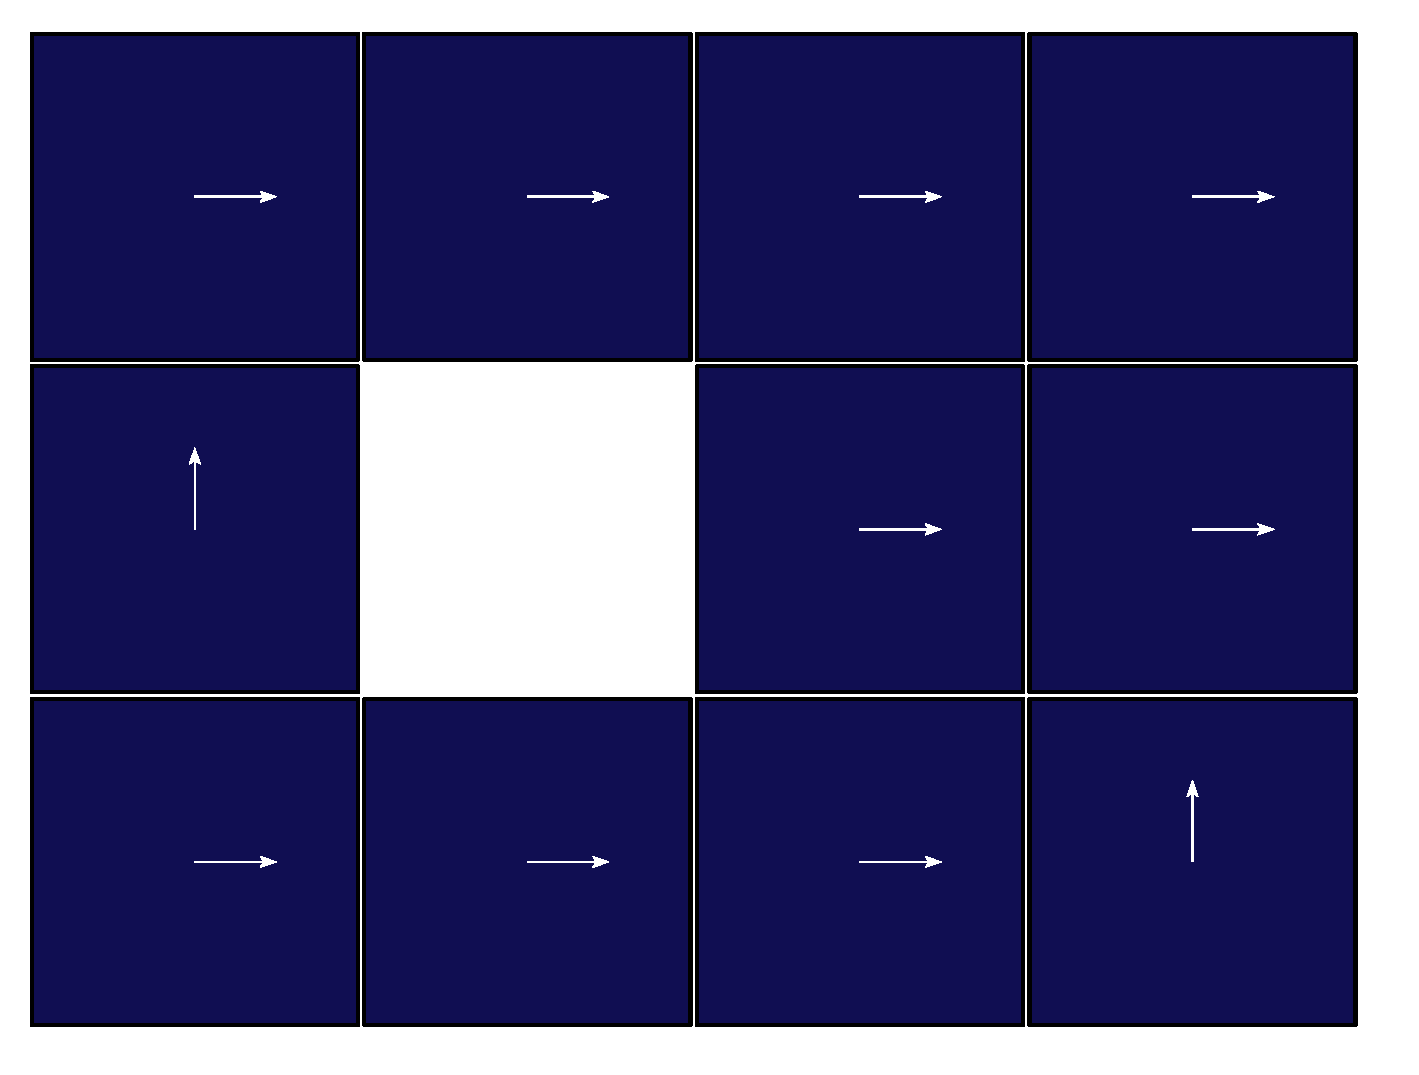
\includegraphics[width=0.7\textwidth]{policy_right_or_up}
  %   \caption{Representation of the policy to evaluate}\label{fig:policy-right-or-up}
  % \end{figure}
